% ESAT link-preview diagram: the velocity-time graph from one of the Physics
% papers' questions. Built by og-images/build_esat.py.
\documentclass[border=12pt]{standalone}
\usepackage{pgfplots}
\pgfplotsset{compat=1.18}
\usetikzlibrary{arrows.meta}
\definecolor{surface}{RGB}{250,249,246}
\definecolor{accent}{RGB}{118,59,67}
\definecolor{tint}{RGB}{241,232,231}
\pagecolor{surface}
\begin{document}
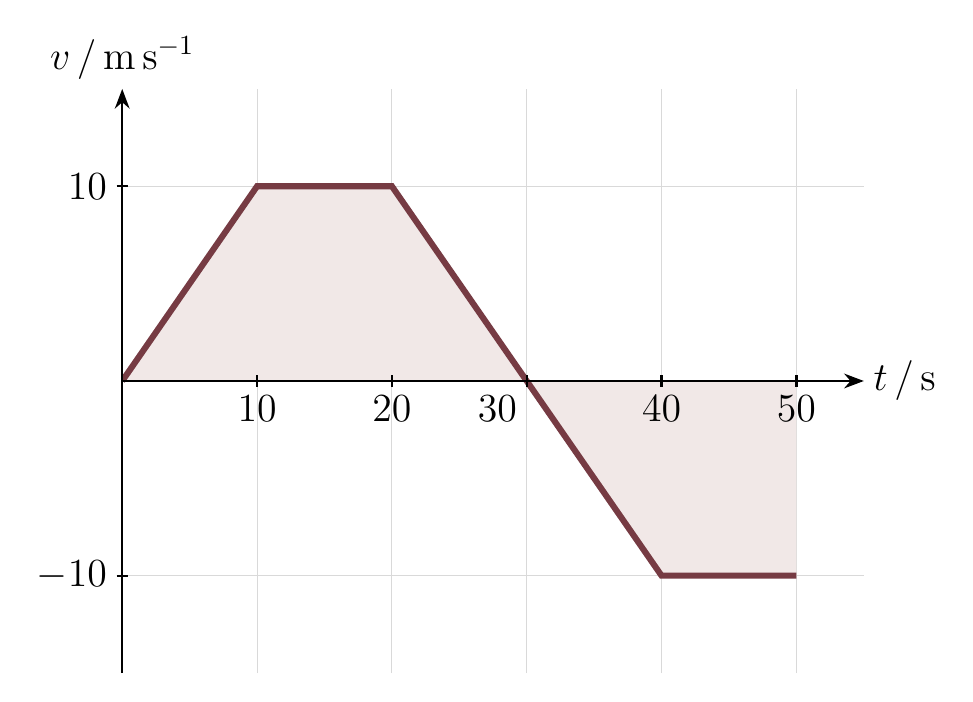
\begin{tikzpicture}[every node/.style={font=\Large}]
\begin{axis}[
    width=11cm, height=9cm,
    tick label style={font=\Large},
    label style={font=\Large},
    axis lines=middle,
    axis on top,
    axis line style={thick, -{Stealth[length=2.5mm]}},
    xmin=0, xmax=55,
    ymin=-15, ymax=15,
    xtick={0,10,...,50},
    ytick={-10,0,10},
    xticklabels={,$10$,$20$,,$40$,$50$},
    yticklabels={$-10$,,$10$},
    xticklabel style={below},
    yticklabel style={left},
    tick style={black, thick},
    major tick length=4pt,
    xlabel={$t\,/\,\mathrm{s}$},
    ylabel={$v\,/\,\mathrm{m\,s^{-1}}$},
    xlabel style={at={(ticklabel* cs:1)}, anchor=west},
    ylabel style={at={(ticklabel* cs:1)}, anchor=south},
    clip=true,
]
\pgfplotsinvokeforeach{10,20,30,40,50}{
    \draw[gray!30] (axis cs:#1,-15) -- (axis cs:#1,15);
}
\pgfplotsinvokeforeach{-10,10}{
    \draw[gray!30] (axis cs:0,#1) -- (axis cs:55,#1);
}
\fill[tint] (axis cs:0,0) -- (axis cs:10,10) -- (axis cs:20,10) -- (axis cs:30,0) -- cycle;
\fill[tint] (axis cs:30,0) -- (axis cs:40,-10) -- (axis cs:50,-10) -- (axis cs:50,0) -- cycle;
\addplot[line width=2.2pt, accent, mark=none] coordinates {(0,0) (10,10) (20,10) (40,-10) (50,-10)};
\node[below left, yshift=-2pt] at (axis cs:30,0) {$30$};
\end{axis}
\end{tikzpicture}
\end{document}
